\chapter{Cơ bản của xử lí số liệu trong vật lí}
\exercise Khoảng cách trung bình từ trái đất đến mặt trời là $1{,}5 \cdot 10^8$ km. Giả sử quỹ đạo của trái đất quanh mặt trời là tròn và mặt trời được đặt tại gốc của hệ quy chiếu.
\begin{enumerate}
   \item Tính tốc độ di chuyển trung bình của trái đất quanh mặt trời dưới dạng dặm trên giờ ($1 \;\text{dặm}=1{,}6093\;\text{km}$).
   \item Ước lượng góc $\theta$ giữa véc-tơ vị trí của trái đất bây giờ và vị trí sau đó $4$ tháng.
   \item Tính khoảng cách giữa hai vị trí đó.
\end{enumerate}
\solution
\begin{enumerate}
   \item Giả sử trái đất quay quanh mặt trời trong $365{,}25$ ngày. Quãng đường mà trái đất đi được trong thời gian này là chu vi của quỹ đạo tròn $2 \pi \cdot 1{,}5 \cdot 10^8$ km. Từ đó, chúng ta có thể tính được tốc độ trung bình của trái đất quanh mặt trời là $\frac{2 \pi \cdot 1{,}5 \cdot 10^8\ \text{km}}{365{,}25\ \text{ngày}}$. Thực hiện quy đổi để được:
      \[
         \frac{2 \pi \cdot 1{,}5 \cdot 10^8\ \text{km}}{365{,}25\ \text{ngày}}
         \cdot \frac{1\ \text{dặm}}{1{,}6903\ \text{km}}
         \cdot \frac{1\ \text{ngày}}{24\ \text{h}}
         = \boxed{6{,}4\cdot 10^4\ \frac{\text{dặm}}{\text{h}}}.
      \]
   \item Trái đất quay quanh mặt trời trong $12$ tháng, tương đương với một góc quay $360^{\circ}$ so với gốc là mặt trời. Coi như các tháng có độ dài như nhau. Ta có $\theta$ chính là góc quay của trái đất trong $4$ tháng, tương đương với:
   \[
      \theta = \frac{360^{\circ}}{12\ \text{tháng}} \cdot 4\ \text{tháng}= \boxed{120^{\circ}}.
   \]
   \item
\end{enumerate}

\begin{wrapfigure}{R}{0.3\textwidth}
   \centering
   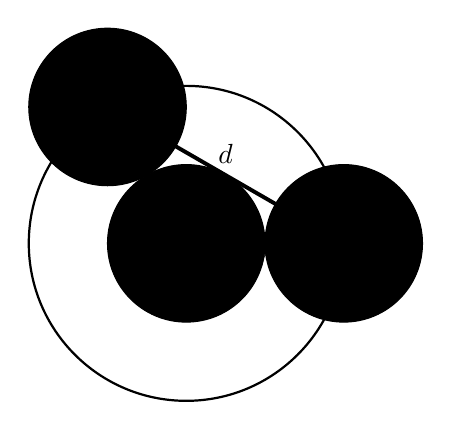
\begin{tikzpicture}
      \draw[thick] (0,0) circle (2cm);
      \filldraw[black] (0,0) circle (\pointSize) node[anchor=north] {O};
      \draw[->, thick, >=latex, line width=0.5mm] (0,0) -- (0:2cm) node[midway, below] {$r$};
      \draw[->, thick, >=latex, line width=0.5mm] (0,0) -- (120:2cm);
      \draw[thick, line width=0.5mm] (0:2cm) -- (120:2cm) node[midway, above] {$d$};
      \filldraw[black] (0:2cm) circle (\pointSize) node[anchor=west] {A};
      \filldraw[black] (120:2cm) circle (\pointSize) node[anchor=south] {B};
      \node at (60:0.3cm) {$\theta$};
      \draw[thick] (0:0.5cm) arc[start angle=0, end angle=120, radius=0.5cm];
   \end{tikzpicture}
   \caption{Quỹ đạo trái đất}
   \label{fig:earth}
\end{wrapfigure}

Gọi $A$ là vị trí của trái đất bây giờ, $B$ là vị trí của trái đất sau $4$ tháng theo như hình \ref{fig:earth}. Coi một đơn vị trên tọa độ bằng độ dài bán kính của quỹ đạo tròn, tức là $r=1{,}5\cdot10^8$ km. Ta có tọa độ điểm $A$ là $(1;0)$. Tọa độ điểm $B$ là $\left(\cos(120^{\circ}); \sin(120^{\circ})\right)=\left(-\frac{1}{2}; \frac{\sqrt{3}}{2}\right)$. Từ đó, chúng ta có khoảng cách giữa hai vị trí đó là: $$d = r\cdot \sqrt{\left(1-\left(-\frac{1}{2}\right)\right)^2 + \left(\frac{\sqrt{3}}{2}\right)^2}=\boxed{2{,}6\cdot10^8\ \text{km}}.$$

\exercise Khối lượng riêng (bằng khối lượng của vật chia cho thể tích của vật đó) của nước là $1{,}00 \;\frac{\text{g}}{\text{cm}^3}$.
\begin{enumerate}
   \item Tính giá trị này theo ki-lô-gam trên mét khối.
   \item $1{,}00$ lít nước nặng bao nhiêu ki-lô-gam, bao nhiêu pao (lb)? Biết $1\ \text{lb} = 0{,}45\ \text{kg}$ (chính xác).
\end{enumerate}

\solution
\begin{enumerate}
   \item Thực hiện quy đổi, chúng ta có:
   \begin{align*}
      1{,}00\;\frac{\text{g}}{\text{cm}^3} &= \left(1{,}00\;\frac{\text{g}}{\text{cm}^3}\right)\cdot\frac{1\ \text{kg}}{1000\ \text{g}}\cdot\left(\frac{100\ \text{cm}}{1\ \text{m}}\right)^3 \\
      &= \boxed{1{,}00\cdot 10^3\ \frac{\text{kg}}{\text{m}^3}}.
   \end{align*}
   \item Khối lượng của $1{,}00$ lít nước là
   \begin{align*}
      1{,}00\ \text{L} \cdot \left(1{,}00\cdot 10^3\ \frac{\text{kg}}{\text{m}^3}\right)&= 1{,}00\ \text{L} \cdot \left(1{,}00\cdot 10^3\ \frac{\text{kg}}{\text{m}^3}\right) \cdot \frac{1\ \text{m}^3}{1000\ \text{L}} \\
      &= \boxed{1{,}00\cdot 10^0\ \text{kg}}.
   \end{align*}
   Theo đơn vị pao (lb), chúng ta có:
   \[
      1{,}00\cdot 10^0\ \text{kg} = 1{,}00\cdot 10^0\ \text{kg} \cdot \frac{1\ \text{lb}}{0{,}45\ \text{kg}} = \boxed{2{,}22\cdot 10^0\ \text{lb}}.
   \]
\end{enumerate}

\exercise Trong hệ thời gian cổ Trung Hoa, từ triều đại Thanh trở về trước (trừ một số năm), một ngày được chia thành $100$ khắc. Sau triều đại này (trừ một số năm), một ngày được chia thành $96$ khắc. Coi một ngày có $24$ giờ và mọi số liệu là chính xác tuyệt đối.
\begin{enumerate}
   \item Tính số giây (hệ đo lường hiện đại) trong một khắc trong cả hai thời kì.
   \item Tính tỉ lệ về độ dài của hai khắc trong hai thời kì.
\end{enumerate}

\solution
\begin{enumerate}
   \item Số giây trong một ngày là $$24\ \text{h} \cdot \frac{60\ \text{phút}}{1\ \text{h}} \cdot \frac{60\ \text{giây}}{1\ \text{phút}} = 86400\ \text{giây}.$$
\end{enumerate}
Từ triều đại Thanh trở về trước, số giây trong một khắc là $$\frac{86400\ \text{giây}}{100\ \text{khắc}_{\text{trước}}} = \boxed{864 \frac{\text{giây}}{\text{khắc}_{\text{trước}}}}.$$
Sau triều đại Thanh, số giây trong một khắc là $$\frac{86400\ \text{giây}}{96\ \text{khắc}_{\text{sau}}} = \boxed{900 \frac{\text{giây}}{\text{khắc}_{\text{sau}}}}.$$
\begin{enumerate}
   \item[2] Tỉ lệ độ dài thời gian một khắc trước và sau là $$\frac{1\ \text{khắc}_{\text{trước}}}{1\ \text{khắc}_{\text{sau}}} = \frac{1\ \text{khắc}_{\text{trước}}}{1\ \text{khắc}_{\text{sau}}}\cdot \frac{864\ \text{giây}}{1\ \text{khắc}_{\text{trước}}}\cdot\frac{1\ \text{khắc}_{\text{sau}}}{900\ \text{giây}}=\boxed{0{,}96}.$$
\end{enumerate}

\exercise Một vòng đĩa tròn như trong hình \ref{fig:vong_dia} có đường kính $4{,}50$ cm rỗng ở giữa một lỗ đường kính $1{,}25$ cm. Đĩa dày $1{,}50$ mm. Biết rằng đĩa được làm từ chất liệu có khối lượng riêng là $8600\;\frac{\text{kg}}{\text{m}^3}$. Tính khôi lượng vòng đĩa theo gram.

\begin{figure}
   \centering
   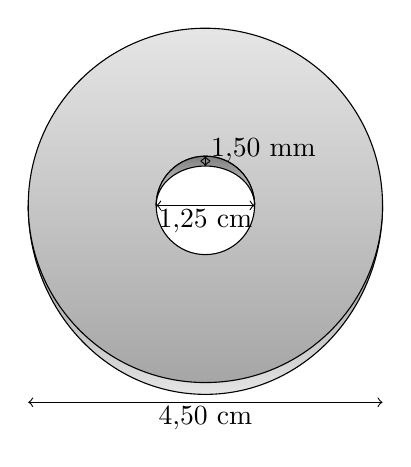
\begin{tikzpicture}
      % Draw the shape
      \draw[bottom color=gray!20] (-2.25, 0) arc[start angle=180, end angle=360, x radius = 2.25cm, y radius = 2.4cm];
      \draw[bottom color=gray!70, top color=gray!20] (0, 0) circle (2.25cm);
      \draw[fill=white] (0, 0) circle (0.625cm);
      \draw[bottom color = gray!20] (-0.625, 0) arc[start angle=180, end angle=0, radius = 0.625cm];
      \draw[fill=white] (-0.625, 0) arc[start angle=180, end angle=0, x radius = 0.625cm, y radius = 0.5cm];
      % Draw the dimension
      \draw[<->] (-2.25,-2.5) -- (2.25,-2.5);
      \node at (0, -2.7) {$4{,}50$ cm};
      \draw[<->] (-0.625,0) -- (0.625,0);
      \node at (0, -0.2) {$1{,}25$ cm};
      \draw[<->] (0,0.5) -- (0,0.625);
      \node[anchor=west] at (-0.05, 0.7) {$1{,}50$ mm};
   \end{tikzpicture}
   \caption{Vòng đĩa tròn}
   \label{fig:vong_dia}
\end{figure}

\solution

Đặt $D=4{,}50\;\text{cm}=4{,}50\times 10^{-2}\ \text{m}$, $d=1{,}25\ \text{cm}=1{,}25\times 10^{-2}\;\text{m}$, $h=1{,}50\ \text{mm}=1{,}50\times 10^{-3}\ \text{m}$ và $\mathcal{D}=8600\;\frac{\text{kg}}{\text{m}^3}=8{,}6\times 10^3\;\frac{\text{kg}}{\text{m}^3}\cdot \frac{10^3\;\text{g}}{\text{kg}}=8{,}6\times 10^6\;\frac{\text{g}}{\text{m}^3}$.

Nhận thấy rằng đĩa có dạng trụ, diện tích mặt đáy là $$S=\pi\cdot \left(\frac{D}{2}\right)^2-\pi\cdot \left(\frac{d}{2}\right)^2=\frac{\pi \left(D^2-d^2\right)}{4}.$$

Thể tích của đĩa là $V=S\cdot h=\frac{\pi \cdot h\cdot \left(D^2-d^2\right)}{4}.$ Nhân với khối lượng riêng, chúng ta có khối lượng của đĩa là $$m=\mathcal{D}\cdot V=\frac{\pi \cdot h\cdot \mathcal{D}\cdot \left(D^2-d^2\right)}{4}.$$ Thay số trực tiếp với sự để ý đến số chữ số có nghĩa, chúng ta có kết quả $m=\boxed{1{,}89\times 10^1\ \text{kg}}$.

\exercise Khối lượng của một chất lỏng được mô hình hóa bởi phương trình $m=A\cdot t^{0{,}8}-B\cdot t$. Nếu như $t$ được tính bằng giây và $m$ được tính bằng ki-lô-gram, thì đơn vị của $A$ và $B$ là gì?

\solution

Để có thể cộng trừ các phần tử, chúng cần phải có cùng đơn vị. Do vậy, đơn vị của $A\cdot t^{0{,}8}$ và $B\cdot t$ là kg. Từ quy tắc nhân chia các đơn vị, chúng ta có:
\begin{equation*}
   \begin{cases}
      A\cdot \text{s}^{0{,}8} &=\text{kg} \\
      B\cdot\text{s} &=\text{kg}
   \end{cases}
   \iff
   \begin{cases}
      A &=\frac{\text{kg}}{\text{s}^{0{,}8}} \\
      B&=\frac{\text{kg}}{\text{s}}
   \end{cases}.
\end{equation*}

Vậy đơn vị của $A$ là $\boxed{\frac{\text{kg}}{\text{s}^{0{,}8}}}$ và đơn vị của $B$ là $\boxed{\frac{\text{kg}}{\text{s}}}$.
